\chapter{Relaterat arbete}
I projektet har metoder och ramverk för såväl arbete som mjukvara använts. Nedan kommer en förklaring på de största delarna som använts och implementerats.

\section{Scrum}
Scrum är ett ramverk som innefattar olika roller, aktiviteter och tekniker för att förenkla utvecklingsprocessen. Det finns nyckelroller inom teamet för att se till att alla delar ses över utan att lägga allt ansvar på en individ. Det finns även en rad förutbestämda möten och uppdateringar som är till för att ge hela gruppen bra överblick och en chans att påverka arbetet.

Inom Scrum delas hela utvecklingsperioden upp i tidsrutor, så kallade sprintar. Dessa är förutbestämda tidsperioder som strukturmässigt är uppbyggda på samma sätt varje omgång. De inleds med ett planeringsmöte där fokus och mål för förestående sprint bestäms. Inför varje ny arbetsdag hålls ett kort scrummöte där alla i teamet får presentera det de gjort sen senast och vad de ska göra kommande arbetsdag. Detta för att alla ska få en bra bild över hur arbetet ligger till tidsmässigt och om det finns några problem som måste lösas. 

I slutet av varje sprint hålls två möten. En sprintgranskning och en sprintåterblick. Sprintgranskningen går ut på att alla i utvecklingsteamet sätter sig ned, eventuellt även med kund, och går igenom vad som åstadkommits under senaste sprint. Arbetet demonstreras och utvecklarna svarar på eventuella frågor, presenterar problem och hur dessa har lösts. Detta möte är till för att utvärdera de tekniska lösningar som applicerats. Sprintåterblicken är ett internt möte för utvecklingsteamet. Även här ska senaste arbetet utvärderas men ur ett socialt perspektiv istället för ett tekniskt. Här ska gruppens relationer diskuteras, hur användandet av valda verktyg fungerat och det finns även tillfälle för alla enskilda individer att utvärdera egen arbetsinsats.

Alla krav som finns för projektet sparas i en så kallad backlogg. Det är en rörlig lista där krav rangordnas utefter prioritet. När ett krav blir mer aktuellt eller mer väldefinierat flyttas det uppåt i listan. \cite{scrumguide}

\section{Mjukvaruramverk}
Två stora mjukvaruramverk som använts i projektet är Ruby on Rails samt Angularjs.

\subsection{Ruby och Ruby on Rails}
Ruby on Rails är ett ramverk skrivet i språket Ruby \cite{rubylang}. Ramverket är skrivet med öppen källkod som används utav flera stora tjänster på nätet, bland annat mikrobloggstjänsten Twitter, sammarbetsverktyget Github och boendeförmedlingstjänsten Airbnb. Ramverket är skrivet enligt designmönstret MVC. Detta står för \textit{model}, \textit{view}, \textit{controller} och är ett sätt att strukturera ett projekts logik på sådant vis att olika komponenter har egna tydliga platser och syften.

I Ruby on Rails skapar utvecklaren \textit{models}. Detta är en samling klasser vars syfte är att hantera data som användaren eller systemet interagerar med, och fungerar som ett lager ovanpå databasen. Ett exempel på en \textit{model} kan vara en klass för användare eller filer. Samtliga databasoperationer sker genom systemets \textit{models}. En \textit{model} skrivs i Ruby med syntaxen \textit{CamelCase} medans klasstabellerna i databasen är namngivna med \textit{snail}\_\textit{case}.

Den komponent som sköter interaktionen mellan det som användaren interagerar med och systemets \textit{models} är systemets \textit{controllers}. Här finns logik för att hantera användares handlingar och hämta data från systemets \textit{models}. Ett exempel kan vara att användaren klickar på en knapp i webbläsaren. Syftet med knappen är att visa en viss data. Användarens handling skickas till en \textit{controller} som tar emot vad det är för data som användaren efterfrågar och hämtar den datan från en \textit{model}. Här finns också logik för att hantera undantag, till exempel om datan saknas. Den \textit{controller} som anropats skickar sedan resultatet av användarens begäran vidare till användaren.

Det som användaren i sin tur interagerar med är systemets \textit{views}. Här presenteras det som systemets \textit{controllers} producerat. Knappen som användaren trycker på, i exemplet i stycket ovan, skapas i en \textit{view}. Här kan det också finnas länkar, texter, textfält och alla andra komponenter som utgör det som renderas av en webbläsare.

En mer överskådlig figur för hur data och interaktioner generellt sett färdas genom ett MVC-system visas i figuren nedan. Data transporteras från \textit{models} till \textit{views} via \textit{controllers}. Interaktioner färdas mellan \textit{views} och \textit{models} via \textit{controllers} och direkt mellan \textit{controllers} och \textit{views} samt mellan \textit{controllers} och \textit{models}, se figur \ref{fig:mvc1}.

\begin{figure}[!H]
\centering
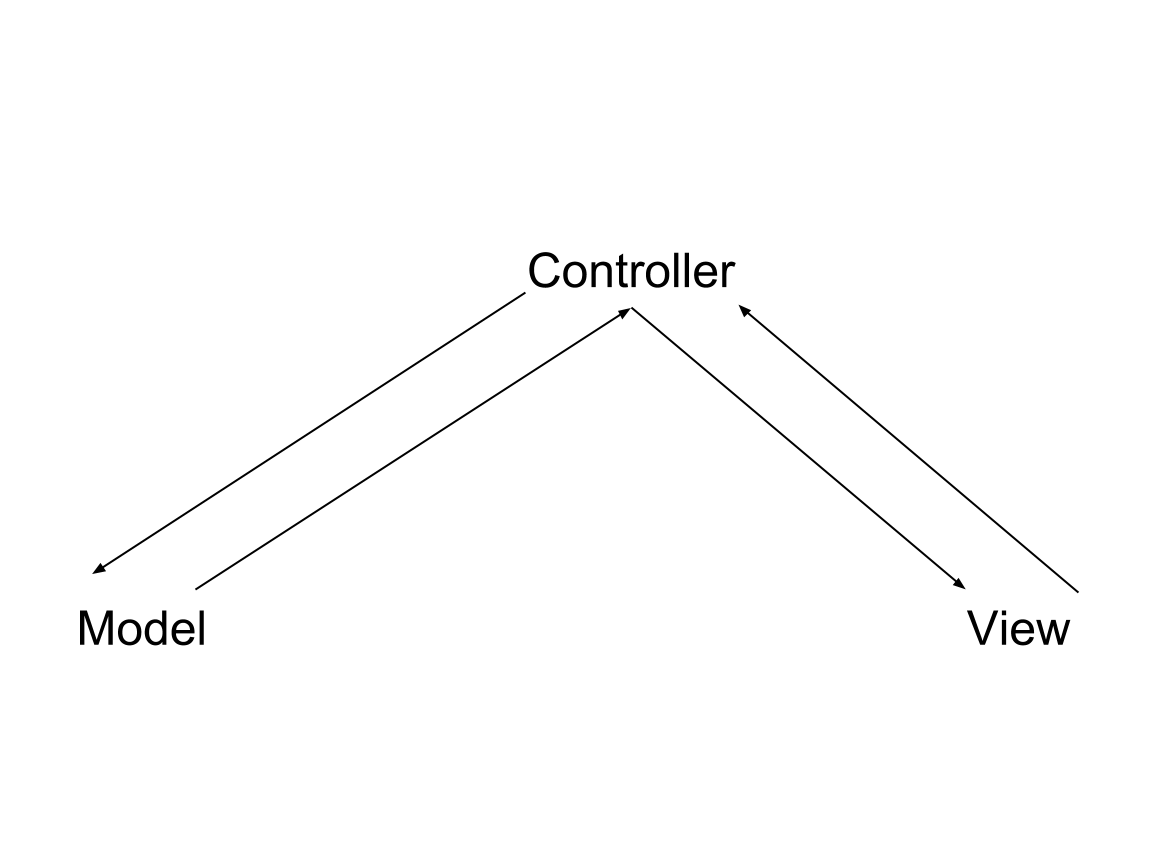
\includegraphics[width=0.8\textwidth]{figures/mvc1.png}
\caption{MVC-systemets struktur.}
\label{fig:mvc1}
\end{figure}

En annan figur som snarare fokuserar på MVC ur ett användarperspektiv visas i figur \ref{fig:mvc2}.

\begin{figure}[!H]
\centering
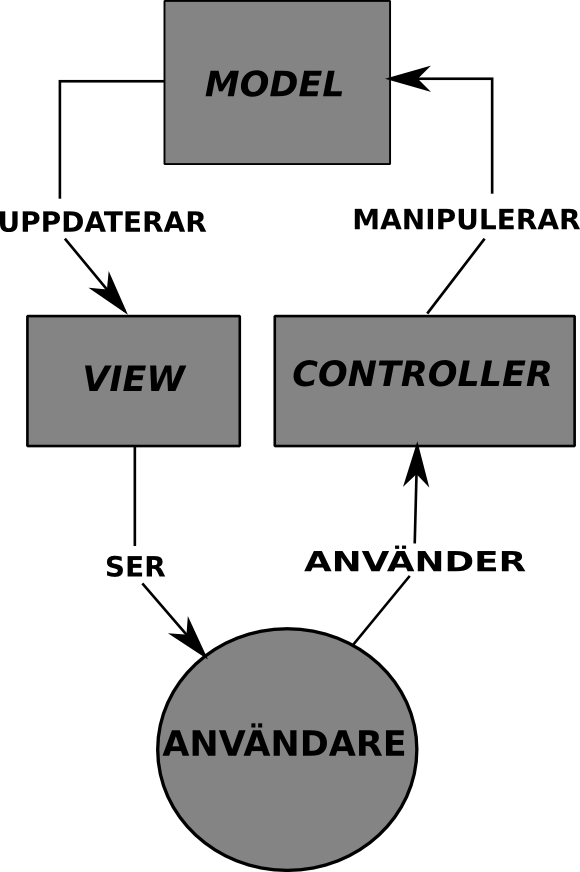
\includegraphics[width=0.8\textwidth]{figures/mvc_user.png}
\caption{MVC ur ett användarperspektiv.}
\label{fig:mvc1}
\end{figure}

\subsection{Angularjs}
Angularjs är ett så kallat MVW-ramverk, vilket står för \textit{Model}-\textit{View}-\textit{Whatever} \cite{angularjs}. För att effektivt använda detta ramverk bör även systemet byggas upp efter den designen. Då \textit{whatever} innebär att det finns flera olika typer av sätt att kontrollera eller manipulera data på, kan varje komponent i systemet få specialanpassade lösningar. 

I Angularjs finns så kallade \textit{factories}. Detta är en samling hjälpfunktioner vars syfte är att undvika kodupprepning och göra det enkelt för koden att återanvändas på flera platser i systemet.

\section{Övrig tredjepartsmjukvara}
Då Ruby on Rails och Angularjs är mjukvara med öppen källkod har det bildats globala nätverk kring dessa ramverk. Många tillägg, verktyg och bibliotek har skrivits för att underlätta utvecklandet i dessa ramverk. 

För att underlätta för utvecklare har Ruby on rails byggts med en mängd olika verktyg. Möjligheten finns även för utvecklare att bygga egna verktyg som kallas för \textit{gems} och är ofta fria att använda och även de skrivna med öppen källkod. 

För att fortsätta bidra till detta nätverk kring Ruby on Rails och Angularjs utvecklades även projektet med öppen källkod, för att kunna dela de lösningar som tagits fram.

\section{Taggar och sökning}
För att uppnå en effektiv sökstruktur i en databas finns det två olika metoder. Den första metoden kallas professionell indexering och är hierarkisk. Den andra metoden kallas folksonomi vilket bygger på att taggar sätts på innehållet utan någon särskild hierarki. Sammanfattat kan de beskrivas som “\emph{Indexering strävar efter precision medan taggning strävar efter hantering}” \cite{tagging}.

Genom professionell indexering ramas den eftersökta informationen in med hjälp av huvudkategorier och underkategorier. Det går alltid att ta sig fram i databasens olika kataloger och till slut hitta den sökta filen. Folksonomi går ut på att hitta den eftersökta filen genom taggar. Nyckelorden behöver inte följa någon speciell hierarki eller struktur sinsemellan.  

\section{Gränssnitt}
För att designa ett användavänligt gränssnitt kan Normans Principer\cite{norman} tillämpas för att åstadkomma en god användarupplevelse. Dessa utgår ifrån sex punkter: synlighet, återkoppling, begränsningar, mappning, konsekvens och affordans.

\subsection{Synlighet}
Det är viktigt att utforma en design som gör att användaren känner sig trygg i gränssnittet. Användaren ska helst kunna förutspå vad som händer när denne klickar på en ikon eller en rubrik. Ikoner ska tala för sig själv, till exempel en ikon med en soptunna betyder kasta och en penna betyder redigera. För att göra det lättare för användaren att hitta det mest relevanta på sidan kan tomma utrymmen användas \cite{whitespace}. Dessa tomma utrymmen är grafiska utrymmen som inte innehåller någon typ av information. De är till för att skapa mer “luft” i gränssnittet. Detta gör att användares fokus begränsas kring ett visst område och det blir lättare att navigera.

\subsection{Återkoppling}
Att ständigt ge återkoppling till vad som sker eller vad som har skett gör att användare känner sig tryggare i systemet. Dialogrutor, laddningssymboler och felmeddelande är exempel på viktig återkoppling \cite{whitespace}. Utan en laddningssymbol kan användaren få känslan av att ingenting händer och går därför kanske tillbaka och upprepar steget, vilket förstör hela processen.

\subsection{Begränsningar}
För att användaren inte ska göra oönskade saker i systemet eller ha för många alternativ, är det en bra idé att begränsa alternativen \cite{whitespace}. Till exempel förvirrar för många menyalternativ på en hemsida. 

\subsection{Mappning}
Mappning innebär att liknande innehåll samlas på samma plats för att hålla en god struktur \cite{whitespace}. Användare ska snabbt kunna hitta filens tillhörande funktioner. Detta kan åstadkommas genom att visa alternativen i anslutning till filerna. 

\subsection{Konsekvens}
För att göra det lättare för användaren att minnas hur denne använde en funktion är det bra att ha en liknade design på hela hemsidan. Det blir lätt rörigt för användren om designen inte följer ett mönster. Att använda sig av samma teckensnitt och färgschema hjälper till att hålla sidan konsekvent \cite{whitespace}.

\subsection{Affordans}
Affordans betyder att ett objekt själv ska kunna beskriva vad det ska användas till. Till exempel är det tydligt att det går att hänga kläder på en klädkrok och ingen ytterligare beskrivning krävs \cite{whitespace}. Samma sak gäller på en hemsida. Användaren ska inte behöva fundera över vad som kommer hända när denne klickar på exempelvis en papperskorg, det vill säga något kommer att raderas.

\section{Databaserat filsystem}
Ett databasbaserat filsystem använder sökning för att hitta filer genom metadata eller nyckelord. De flesta filsystem använder kataloglagring. Ett examensarbete på University of Twente i Nederländerna hade som uppgift att undersöka om ett databasbaserat filsystem kan ersätta filsystem med kataloglagring med avseende på användbarhet och förmåga att lära sig att använda systemet \cite{twente}. Genom användartester drogs slutsatsen att ett databasbaserat filsystem presterade bättre utifrån dessa aspekter.
